\section{АКТУАЛЬНОСТЬ ТЕМЫ}

Турбулентность остается одним из наиболее сложных объектов исследования механики жидкости и газа. За почти столетнюю историю ее изучения предложены десятки различных подходов, почти всегда отражающие наиболее активно развиваемые перспективные направления математики и физики соответствующего периода времени. Статистическая физика и теория вероятности, теория размерности, математический анализ и прямые численные методы, теория динамических систем, теория фракталов - вот далеко не полный перечень областей науки, которые давали основные идеи исследователям турбулентности. Примером турбулентности могут выступать самые обычные потоки воздуха, обтекающие объект, представленные на рисунке \ref{fig:actuality}. Поток воздуха при варьирующихся параметрах ведёт себя по-разному.

\begin{figure}
    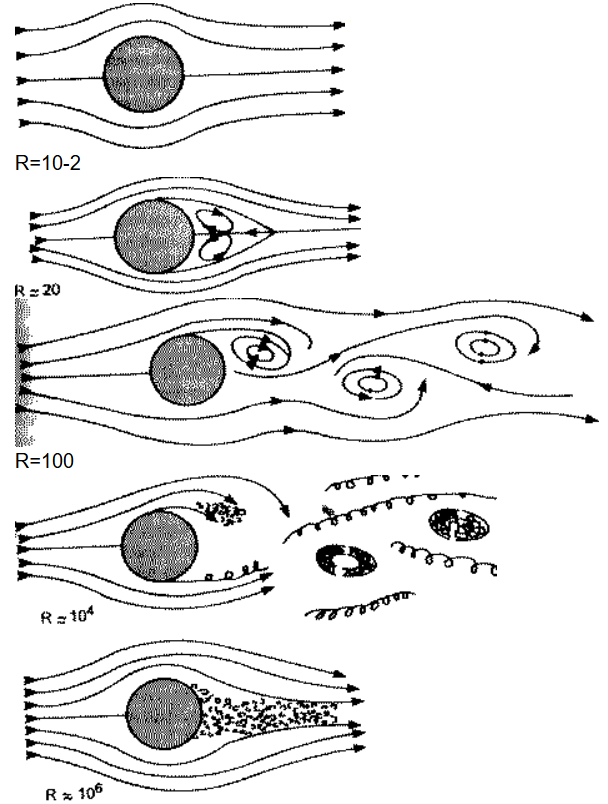
\includegraphics[width=10cm]{2-00-turb_example}
    \caption{Примеры турбулентных потоков при разном критерии Рейнольдса}
    \label{fig:actuality}
\end{figure}

В качестве объекта исследования выбраны течения свободных струй газа, которые наблюдаются в энергетических установках таких как реактивные двигатели, камеры сгорания промышленных печей, горелочные устройства, испытательные стенды и т. д.. На рисунке \ref{fig:actuality2} изображена примерная схема таких установок.

\begin{figure}
    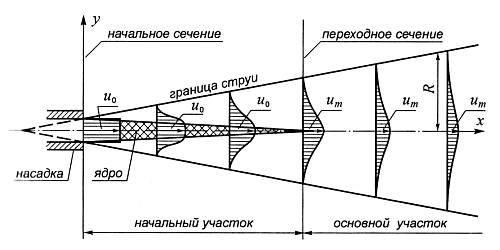
\includegraphics[width=15cm]{2-00-our_task}
    \caption{Объект исследования}
    \label{fig:actuality2}
\end{figure}

В связи с исключительной практической важностью надёжного расчётного предсказания характеристик сложных турбулентных течений для многих областей науки и техники (большинство представляющих интерес течений являются турбулентными), построению таких моделей, разработке методов расчета и проведению численных исследований различных течений на их основе посвящено огромное число работ.
